\documentclass[a4paper, 12pt]{article}
\usepackage[a4paper, top = 1.5cm, bottom = 1.5cm, left = 1cm, right = 1cm]{geometry}
\usepackage[english, russian]{babel}
\usepackage{graphicx}
\usepackage{mathtools}
\usepackage{amsfonts}
\usepackage{subcaption}
\title{Лабораторная работа № 3.5.1 "Изучение плазмы газового разряда в неоне"}
\author{Кирилл Шевцов Б03-402}
\date{16.09.2025}
\begin{document}
\maketitle
\section*{Цель работы}
Изучить вольт-амперную характеристику тлеющего разряда, изучить свойства плазмы методом зондовых
характеристик.
\section*{Оборудование}
Стеклянная газоразрядная трубка, наполненная неоном, источник напряжения, делитель напряжения, потенциометр,
амперметр, вольтметры, амперметры, переключатели.
\section*{Лабораторная установка}
Стеклянная газоразрядная трубка имеет ненагреваемый полый катод, три анода и геттерный узел - стеклянный баллон,
на внутреннюю поверхность которого напылена газопоглощающая плёнка (геттер). Трубка наполнена изотопом неона при давлении
2 мм. рт. столба. Катод и один из анодов с помощью переключателя $P_{1}$ подключаются через балластный резистор
$R_{b}$ к регулируемому ВИП.
\begin{figure}[htbp]
    \centering
    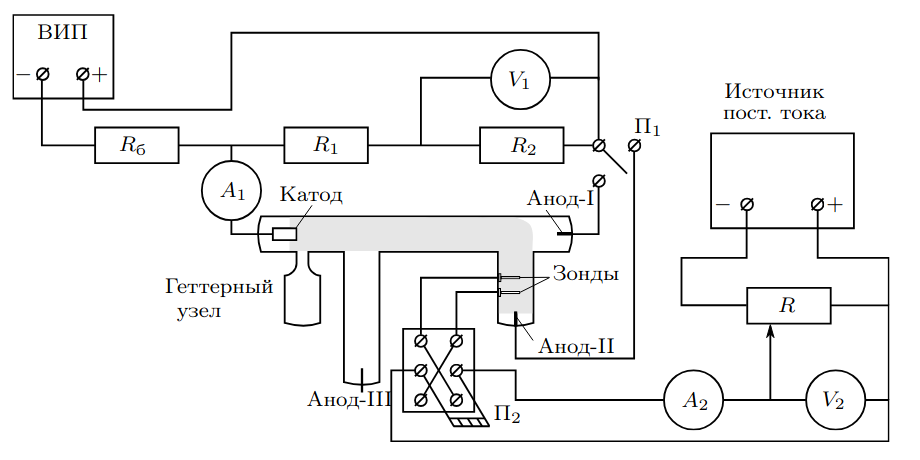
\includegraphics[width=0.6\linewidth]{p1.png}
    \caption{установка для исследования газового разряда}
    \label{установка для исследования газового разряда}
\end{figure}
При подключении первого анода к ВИП, между ним и катодом возникает газовый разряд. Ток разряда измеряется
амперметром $A_{1}$, падение напряжения - на вольтметре $V_{1}$, подключенным к трубке через делитель напряжения с
коэффициентом, равным $\alpha = {R_{1} + R_{2}}/R_{2} = 10$. При подключении к ВИП второго анода, возникает газовый разряд между
катодами и вторым анодом, где находится двойной зонд, необходимый для диагностики плазмы. Третий анод в работе не используется.
\section*{Необходимые формулы}
Частота коллективных колебаний электронов (или плазменная частота) относительно квазинейтрального состояния (то есть такого состояния, при котором равна нулю средняя
плотность заряда):
\begin{equation}
    \omega_{p} = \sqrt{\frac{4\pi n_{e}e^{2}}{m_{e}}}
    \label{частота коллективных колебаний}
\end{equation}
колебания, описываемые плазменной частотой, называют ленгмюровскими.\newline
Важнейшний плазменный параметр, задающий характерный пространственный масштаб многих плазменных явления - дебаевский радиус:
\begin{equation}
    r_{D} = \sqrt{\frac{k_{B}T_{e}}{4\pi n_{e}e^{2}}}
    \label{дебаевский радиус основной}
\end{equation}
Эти два  параметра представляют собой две важные характеристики плазмы, определяющие временной и пространственный масштабы коллективного
движения электронов относительно ионов.
\textbf{Замечание:} если плазма неравновесная, различают два типа дебаевской длины: электронную (\ref{электронная дебаевская длина}) и ионную (\ref{ионная дебаевская длина}),
в понимании, что их температуры различны $T_{e} \neq T_{i}$:
\begin{subequations}
    \begin{equation}
        r_{De} = \sqrt{\frac{k_{B}T_{e}}{4\pi n_{e}e^{2}}}
        \label{электронная дебаевская длина}
    \end{equation}
    \begin{equation}
        r_{Di} = \sqrt{\frac{k_{B}T_{i}}{4\pi n_{i}e^{2}}}
        \label{ионная дебаевская длина}
    \end{equation}
\end{subequations}
Поэтому иногда дебаевский радиус называют поляризационной длиной.\newline
Выражение, определяющее энергию кулоновского взаимодействия частиц в плазме:
\begin{equation}
    \varphi = -\frac{q}{\tilde{r}}\exp\left(-\frac{r}{r_{D}}\right)
    \label{энергия кулоновского взаимодействия}
\end{equation}
где $\varphi_{0} = q/\tilde{r}$ - потенциал одного иона.\newline
Плотность энергии кулоновского взаимодействия зарядов в плазме:
\begin{equation}
    \omega = -\frac{1}{2}n_{i}\frac{q^2}{r_{D}}
    \label{плотность энергии кулоновского взаимодействия}
\end{equation}
В сравнении полученной кулоновской энергии с тепловой $l \sim n_{i}kT$:
\begin{equation}
    \frac{l}{\omega} \sim \frac{kTr_{D}}{q^2} = 4\pi n_{i}r^3_{D}
    \label{отношение энергий}
\end{equation}
Отсюда выражение для числа заряженных частиц в сфере дебаевского радиуса (дебаевской сфере):
\begin{equation}
    N_{D} = \frac{4}{3}\pi n_{i}r^3_{D}
    \label{число заряженных частиц в дебаевской сфере}
\end{equation}
Оценка тока насыщения для ионов, согласно полуэмпирическому соотношению Д. Бомома:
\begin{equation}
    I_{in} \sim 0.4n_{i}eS\sqrt{\frac{2kT_{e}}{m_{i}}}
    \label{ток насыщения}
\end{equation}
Зависимость тока от напряжения для ВАХ газового разряда:
\begin{equation}
    I = I_{0}\th\frac{eU}{2k_{B}T_{e}}
    \label{зависимость тока от напряжения для двойного зонда}
\end{equation}
Эту формулу можно использовать для определения температуры электронов по вольт-амперной характеристике двойного зонда.
По пересечению асимптот с вертикальной осью можно определить ток насыщения $I_{in}$, а затем и концентрацию заряженных частиц в плазме.
\section*{Измерения и снятие данных}
\begin{enumerate}
    \item Настроим установку для ВАХ газового разряда согласно инструкции, плавно увеличивая напряжение на ВИП, запишем напряжение
    зажигания, показание вольтметра $V_{1}$. показания выходного напряжения $U_{out}$, входного $U_{in} = \alpha U_{out}$:
    \begin{center}
        \begin{tabular}{|c|c|c|c|c|c|}
            \hline
            Номер измерения & 1 & 2 & 3 & 4\\
            $U_{out}$, В & $152.52$ & $149.54$ & $152.51$ & $152.53$\\
            $U_{in}$, В & 1535.2 & 1495.4 & 1525.1 & 1525.3\\
            \hline
            $\Delta U_{in}$, В & \multicolumn{4}{|c|}{0.1}\\
            $\Delta U_{out}$, В & \multicolumn{4}{|c|}{0.01}\\
            \hline
        \end{tabular}
    \end{center}
    \item С помощью вольтметра $V_{1}$ и амперметра $A_{1}$ измерим ВАХ газового разряда $I(U)$. Ток изменяется в диапазоне $0.5 - 5.0$ мА.
    \begin{center}
        \begin{tabular}{|c|c|c|c|c|c|c|c|c|c|c|c|}
            \hline
            $I$, мА & 0.55 & 0.93 & 1.55 & 2.14 & 2.55 & 3.07 & 3.53 & 4.07 & 4.51 & 5.09\\
            $U$, В & 34.00 & 32.60 & 31.32 & 23.69 & 20.70 & 18.05 & 16.35 & 15.72 & 15.19 & 14.43\\
            \hline
            $I$, мА & 4.50 & 4.02 & 3.53 & 3.00 & 2.53 & 2.03 & 1.55 & 1.04 & 0.54 & -\\
            $U$, В & 15.10 & 15.60 & 16.26 & 18.33 & 20.70 & 24.70 & 31.26 & 32.30 & 34.24 & -\\
            \hline
        \end{tabular}
    \end{center}
    \item Построим график вольт-амперной характеристики газового разряда (рис. \ref{sub@вах газового разряда}). Определим дифференциальное сопротивление:
    \begin{align}
        R_{dif} = 123 \pm 234\ \text{Ом} \quad \delta R_{dif} = 234\ \text{Ом}
    \end{align}
    Построенный график соответствует участку Д-Г графика - поднормального тлеющего разряда:
    \begin{figure}[htbp]
        \centering
        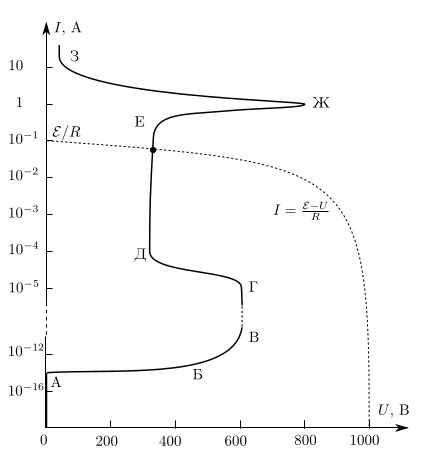
\includegraphics[width=0.4\linewidth]{current.png}
    \end{figure}
    \item Подготовим установку для анализа зондовой характеристики разряда. Снимем ВАХ двойного зонда, плавно увеличивая напряжение
    от $-U_{0}$ до $U_{0}$ при фиксированном токе разряда $I_{p}$. Построим график зондовых характеристик для разных разрядных токов
    (см. рис. \ref{sub@вах двойного зонда})
    \begin{center}
        \centering
        \begin{tabular}{|c|c|c|c|c|c|c|c|c|c|c|c|}
            \hline
            $I_{p}$, мА & \multicolumn{11}{|c|}{$5.000\pm 0.001$}\\
            \hline
            $I$, мА & 22.98 & 22.10 & 21.17 & 20.25 & 19.26 & 18.17 & 17.25 & 15.88 & 12.90 & 6.89 & 0.07\\
            $U$, В & 24.99 & 22.07 & 19.02 & 16.11 & 13.08 & 10.11 & 8.09 & 6.08 & 4.03 & 2.06 & 0.55\\
            \hline
            $I$, мА & -2.66 & -6.74 & -12.96 & -15.90 & -17.13 & -18.19 & -19.38 & -20.37 & -21.34 & -22.33 & -23.18\\
            $U$, В & 0.00 & 2.02 & 4.07 & 6.20 & 8.08 & 10.13 & 13.04 & 16.04 & 19.08 & 22.19 & 24.99\\
            \hline
            $I_{p}$, мА & \multicolumn{11}{|c|}{$4.005\pm 0.001$}\\
            \hline
            $I$, мА & 19.67 & 18.97 & 18.12 & 17.35 & 16.50 & 15.54 & 14.70 & 13.42 & 10.85 & 5.61 & 0.12\\
            $U$, В & 24.99 & 22.11 & 19.09 & 16.12 & 13.09 & 10.07 & 8.01 & 6.01 & 4.08 & 2.08 & 0.60\\
            \hline
            $I$, мА & -0.15 & -5.71 & -10.78 & -13.37 & -14.62 & -15.34 & -16.29 & -17.17 & -18.00 & -18.76 & -19.56\\
            $U$, В & 0.6 & 2.11 & 4.08 & 6.07 & 8.19 & 10.02 & 13.01 & 16.10 & 19.14 & 22.08 & 25.00\\
            \hline
            $I_{p}$, мА & \multicolumn{11}{|c|}{$3.101\pm 0.001$}\\
            \hline
            $I$, мА & 15.92 & 15.31 & 14.65 & 14.00 & 13.28 & 12.37 & 11.68 & 10.45 & 8.05 & 3.98 & 0.05\\
            $U$, В & 24.99 & 22.02 & 19.09 & 16.22 & 13.12 & 10.12 & 8.10 & 6.03 & 4.04 & 2.07 & 0.58\\
            \hline
            $I$, мА & -0.04 & -3.82 & -8.03 & -10.41 & -11.56 & -12.26 & -13.07 & -13.75 & -14.42 & -15.07 & -15.70\\
            $U$, В & 0.58 & 2.01 & 4.06 & 6.07 & 8.12 & 10.10 & 13.24 & 16.09 & 19.11 & 22.18 & 24.99\\
            \hline
            $I_{p}$, мА & \multicolumn{11}{|c|}{$1.513\pm 0.001$}\\
            \hline
            $I$, мА & 9.05 & 8.65 & 8.27 & 7.82 & 7.42 & 6.93 & 6.42 & 5.52 & 4.07 & 1.94 & 0.13\\
            $U$, В & 24.99 & 22.01 & 19.06 & 16.04 & 13.09 & 10.12 & 8.09 & 5.97 & 4.02 & 2.11 & 0.56\\
            \hline
            $I$, мА & -0.13 & -1.88 & -4.06 & -5.52 & -6.37 & -6.84 & -7.34 & -7.73 & -8.16 & -8.56 & -8.95\\
            $U$, В & 0.56 & 2.06 & 4.05 & 6.03 & 8.09 & 10.14 & 13.18 & 16.10 & 19.06 & 22.02 & 24.99\\
            \hline
        \end{tabular}
    \end{center}
    \item По каждой зондовой характеристике определим ионный ток насыщения, наклон характеристики $dI/dU$ в начале координат.
    \item По результатам предыдущего пункта рассчитаем температуру электронов $T_{e}$, концентрацию электронов и ионов в плазме. Считам площадь
    поверхности зонда равной $S \approx \pi dl$, необходимые параметры указаны на установке.
    \item Рассчитаем плазменную частоту колебаний $\omega_{p}$, электронную поляризационную длину $r_{D_{e}}$ и дебаевский радиус экранирования $r_{D}$.
    \item Оценим степень ионизации плазмы, считая давление в трубке $P \approx 2$ торр.
    \item Построим графики зависимости $T_{e}(I_{p})$, $n_{e}(I_{p})$.
\end{enumerate}
\section*{Графики полученных измерений}
\begin{figure}[htbp]
    \centering
    \begin{subfigure}{0.45\textwidth}
        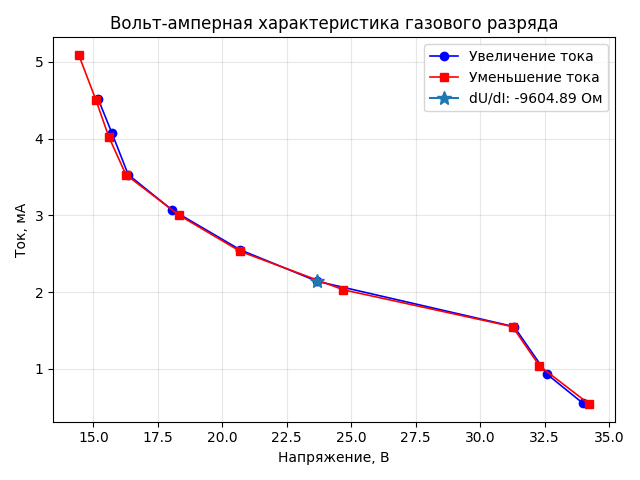
\includegraphics[width=\linewidth]{vax.png}
        \caption{вах газового разряда}
        \label{вах газового разряда}
    \end{subfigure}
    \begin{subfigure}{0.45\textwidth}
        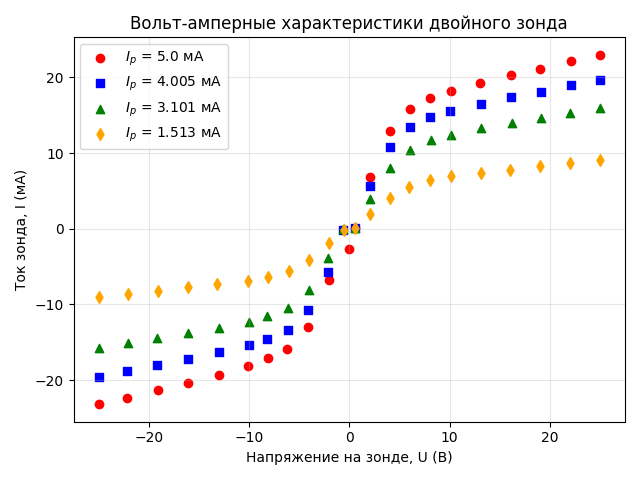
\includegraphics[width=\linewidth]{zond.png}
        \caption{вах двойного зонда}
        \label{вах двойного зонда}
    \end{subfigure}
    \caption{графики $T(n)$ и $\mathcal{M}(n)$}
    \label{графики моментов и периодов}
\end{figure}
\section*{Вывод}
\end{document}
% \begin{figure}[htbp]
    %     \centering
    %     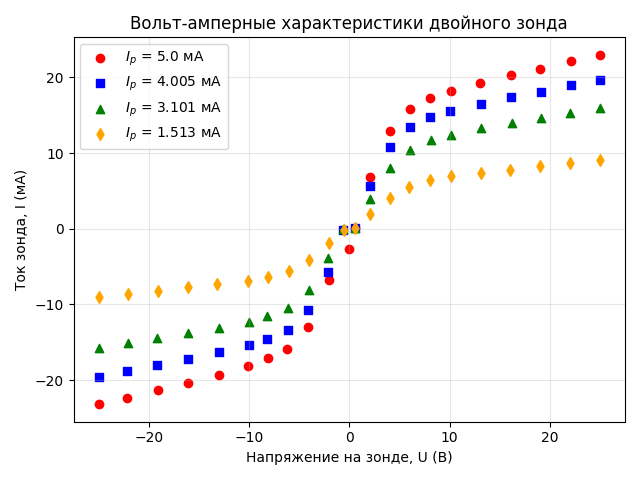
\includegraphics[width=0.8\linewidth]{zond.png}
    %     \caption{зондовые характеристики для разных токах разряда}
    %     \label{зондовые характеристики для разных токах разряда}
    % \end{figure}
    % \item Построим ВАХ разряда в координатной сетке. По наклону кривой определим максимальное дифференциальное сопротивление $R_{dif} = \frac{dU}{dI}$ (см. рис. \ref{})
    % Для этого возьмем две точки графика, для которых прямая проходит под наименьшим наклоном, тогда $R_{dif} \approx 0.031$ Ом.
    % % \begin{figure}[htbp]
    %     \centering
    %     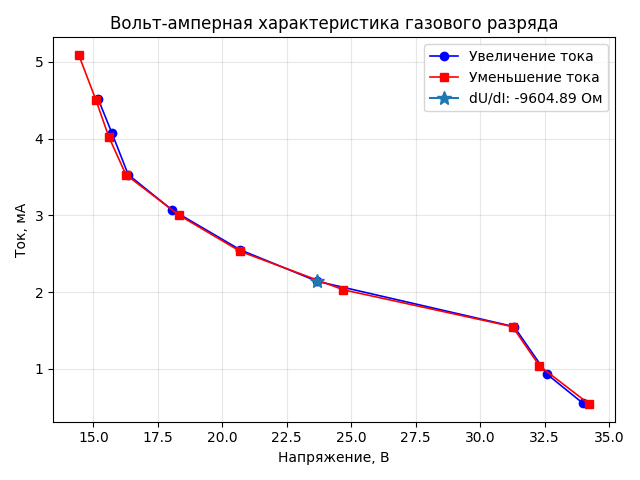
\includegraphics[width=0.8\linewidth]{vax.png}
    %     \caption{ВАХ газового разряда}
    %     \label{ВАХ газового разряда}
    % \end{figure}